\section{Durchführung}
\label{sec:Durchführung}

In dem Experiment werden verschiedene Geräte genutzt um präzise Messergebnisse zu erzielen.
Für die Pumpentechnik wird die Drehschieberpumpe von Pfeiffer Duo 004A mit einem Saugvermögen von 1,1 l/s betrieben.
Für die Messungen im Hochvakuum wird mit der Turbomolekularpumpe SST81 von ILMVAC, betrieben bei 1350 Hz 
mit einem Saugvermögen von 77 l/s, gearbeitet. Bei der Messung der Vakuumwerte kommen drei verschiedene 
Messgeräte zum einsatz. Das Thermovac TR205 (Penning) und die Glühkathode Ionivac IM210, beide von Leybold-Heraeus
sowie die Kaltkathode PKG020 von Balzer.


\begin{figure}
    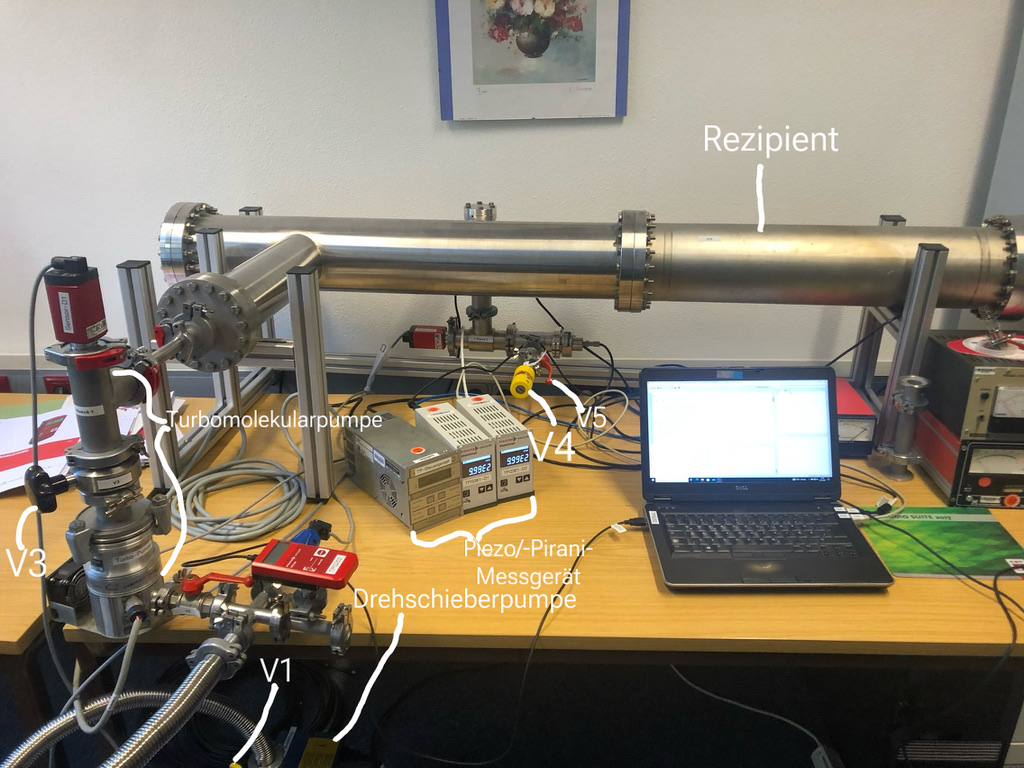
\includegraphics[width=\textwidth]{bilder/Aufbau.jpeg}
    \caption{Der Aufgebaute Versuch inklusive des zusätzlichen Rohres}
\end{figure}


\subsection{Turbomolekularpumpe}
\subsubsection{Evakuierungskurve}


Um die Evakuierungskurve zu bestimmen wird zuerst das schwarze Vential V3 geöffnet.
Vorab musste sichergestellt werden, dass bereits Drücke im Bereich des Hochvakuums erreicht wurden.
Die Messwerte werden  mit einem Pirani-Vakuummeter aufgenommen.
Dieses wird in Betrieb genommen, sobald die Turbomolekularpumpe eine Drehzahl von 1350 Hz erreicht hat.
Um die Kurve zu bestimmen wird das gelbe Dosiervential auf $5\cdot 10^{-6}$bar eingestellt, dabei soll die Pumpe bereits laufen.
Das Kugel und das Nadelvential werden dann zeitgleich geschlossen und über einen Zeitraum von 120sek werden Werte
aufgenommen. Diese werden direkt auf einen angeschlossenen Computer gesendet und abgelsen.
Die Messung wird drei mal durchgeführt. 

\subsubsection{Leckratenmessung}
Um die Leckraten zu bestimmen, ist das Ventil V3 geöffnet, mithilfe des Dosierventils werden vier verschiedene 
Gleichgewichtsdrücke eingestellt. Sobald diese eingestellt sind wird das Ventil V3 geschlossen. Die Werte um welche der Druck
im Laufe der Messzeit bei 120 Sek steigt werden wieder an den Computer gesendet. Die Gleichgewichtsdrücke sind:
$5\cdot 10^{-8}$ bar, $7\cdot 10^{-8}$ bar, $1\cdot 10^{-7}$ und $2\cdot 10^{-7}$ bar.

\subsubsection{Leckraten mit einem dünnen Verbindungsrohr}
Vor der Turbomolekularpumpe wird für die letzten zwei Messungen ein dünnes Rohr eingebaut. Sobald der Druck wieder Werte erreicht hat in 
welchen die Pumpe arbeiten kann wird jeweils für $5\cdot 10^{-8}$ bar und für $2\cdot 10^{-7}$ bar eine weitere Leckratenmessung durchgeführt.


\subsection{Drehschieberpumpe}
\subsubsection{Evakuierungskurve}

Die Bestimmung der Evakuierungskurve der Drehschieberpumpe läuft nach dem selben Prinzip ab. Das gelbe Dosierventil wird geöffnet,
und der Rezipient bei laufender Pumpe mit dem Belüftungsventil V4 kurz belüftet. Die Messung beginnt, sobal das Ventil wieder geschlossen
ist. Der Druckabfall wird 600sek lang von einem Computer aufgenommen, bei diesem Experiment wird ein Kombiniertes Piezo-/Pirani-Messgerät
verwendet. Diese Messung findet einmal statt.

\subsubsection{Leckratenmessung}
Um ein Leck zu simulieren wird bei laufender Pumpe mithilfe des Dosierventils V5 ein Gleichgewichtsdruck im Rezipienten eingestellt.
Es werden sechs Messung durchgeführt, jeweils 200 Sek lang. Die Messung startet, sobald V1 geschlossen wird. Die dabei eingestellten 
Gleichgewichtsdrücke sind $5\cdot 10^{-4}$ bar, 0,01 bar, 0,05 bar und 0,1 bar. Die Messsung bei 0,1 bar wird dabei dreimal durchgeführt.





